\section{Ripasso}
\subsection{Trigonometria}
\[
    sin^2(x) + cos^2(x) = 1
\]
\[
    sin(2x) = 2sin (x)cos(x)
\]
\[
    sin(x) cos(x) = \frac{1}{2}sin(2x)
\]
\[
    cos(2x) = \begin{cases}
        cos^2(x) -sin^2(x)\\
        1-2sin^2(x)\\
        2cos^2(x)-1
    \end{cases}
\]
\[
    sin^2(x) = \frac{1}{2} (1-cos(2x)) \;\;\;\; ottenuta \; da \;[cos(2x) = cos^2(x) - sin^2(x) = 1 - 2 sin^2(x)]
\]
\[
    cos^2(x) = \frac{1}{2}(1+cos(2x)) \;\;\;\; ottenuta \; da \; [cos(2x) = cos^2(x) - sin^2(x) = 2cos^2(x) - 1]
\]
\[
    sin(cos^{-1}(x)) = \sqrt{1-x^2}
\]
\[
    cos(sin^{-1}(x) = \sqrt{1-x^2}
\]
\[
    Ch^(x) = \frac{e^x + e^{-x}}{2}
\]
\[
    Sh^(x) = \frac{e^x - e^{-x}}{2}
\]
\[
    Ch^2(x) - Sh^2(x) = 1
\]
\[
    Sh(2x) = 2Sh(x)Ch(x)
\]
\[
    Ch(2x) = Sh^2(x) + Ch^2(x)
\]
\[
    SettSh(x) = log(+ + \sqrt{x^2+1})
\]
\[
    SettCh(x) = log(x + \sqrt{x-1} \cdot \sqrt{x+1})
\]
\[
    Sh(SettCh(a))= \sqrt{a^2-1} \;\;\;\; ottenuta \; da \; [Ch^2(x) -Sh^2(x) = 1] \rightarrow [Sh(x) = \sqrt{Ch^2(x) -1}] \rightarrow [x = SettCh(a)]
\]
\[
    Ch(SettSh(a))=\sqrt{a^2+1} \;\;\;\; ottenuta \; da \; [Ch^2(x) -Sh^2(x) = 1] \rightarrow [Ch(x) = \sqrt{1 + Sh^2(x)}] \rightarrow [x = SettSh(a)]
\]
\[
    sin(a)cos(b)=\frac{1}{2}sin(a+b)+sin(a-b)
\]
\[
    cos(a)sin(b)=\frac{1}{2}sin(a+b)-sin(a-b)
\]
\[
    cos(a)cos(b)=\frac{1}{2}cos(a+b)+cos(a-b)
\]
\[
    sin(a)sin(b)=-\frac{1}{2}cos(a+b)- cos(a-b)
\]
\[
    sin(a+b) =sin(a)cos(b) + sin(b) cos(a)
\]
\[
    sin(a-b) = sin(a)cos(b) - sin(b)cos(a)
\]
\[
    cos(a+b) = cos(a)cos(b) - sin(a)sin(b)
\]
\[
    cos(a-b)=cos(a)cos(b) + sin(a)sin(b)
\]
\[
    sin(\alpha) + sin(\beta) = 2 sin\left(\frac{\alpha + \beta}{2}\right) cos \left(\frac{\alpha - \beta}{2}\right)
\]
\[
    sin(\alpha) - sin(\beta) = 2 cos\left(\frac{\alpha + \beta}{2}\right) sin\left(\frac{\alpha - \beta}{2}\right)
\]
\[
    cos(\alpha) + cos(\beta) = 2 cos\left(\frac{\alpha + \beta}{2}\right) cos\left(\frac{\alpha - \beta}{2}\right)
\]
\[
    cos(\alpha) - cos(\beta) = -2sin\left(\frac{\alpha + \beta}{2}\right) sin\left(\frac{\alpha - \beta}{2}\right)
\]
\begin{figure}[h!]
    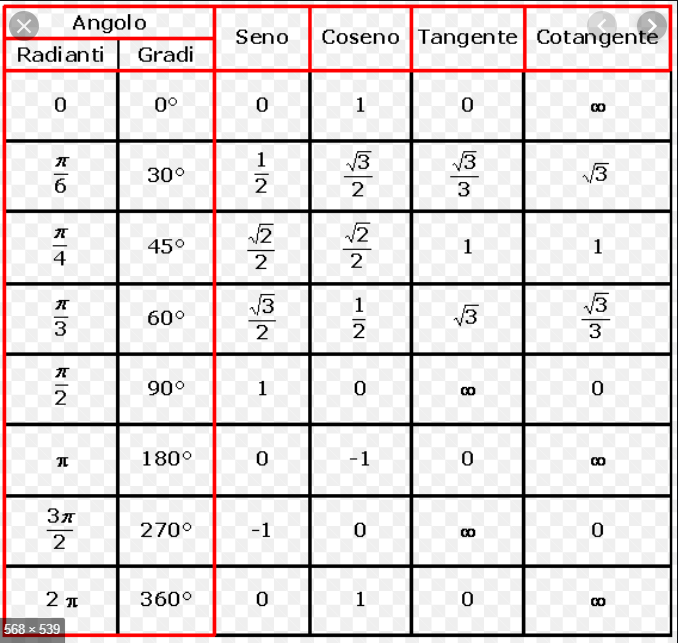
\includegraphics[width=300px]{../0-ripasso/trigonometria.PNG}
\end{figure}
\newpage
\subsection{Asintotici}
\begin{figure}[h!]
    
\includegraphics[width=\linewidth]{../0-ripasso/asintotici.PNG}
\end{figure}
\newpage
\subsection{Derivate}
\begin{figure}[h!]
    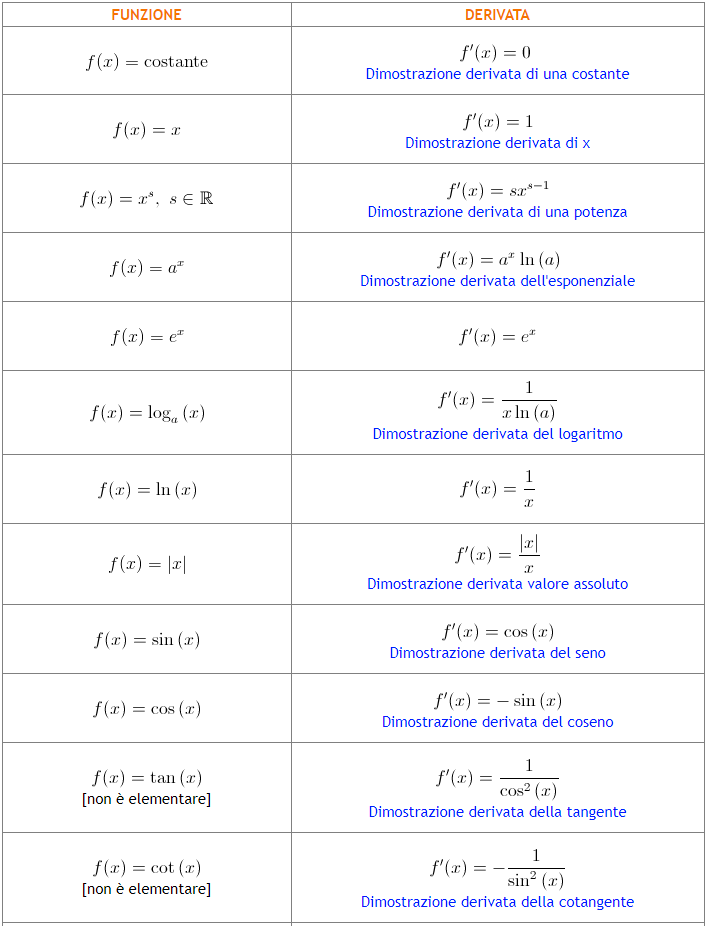
\includegraphics[width=\linewidth]{../0-ripasso/derivate1.PNG}
\end{figure}
\newpage
\begin{figure}[h!]
    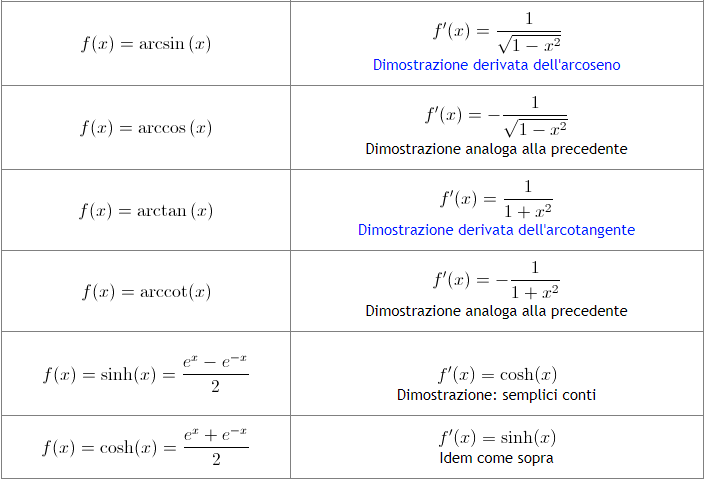
\includegraphics[width=\linewidth]{../0-ripasso/derivate2.PNG}
\end{figure}
\newpage
\subsection{Sviluppi}
\begin{figure}[h!]
    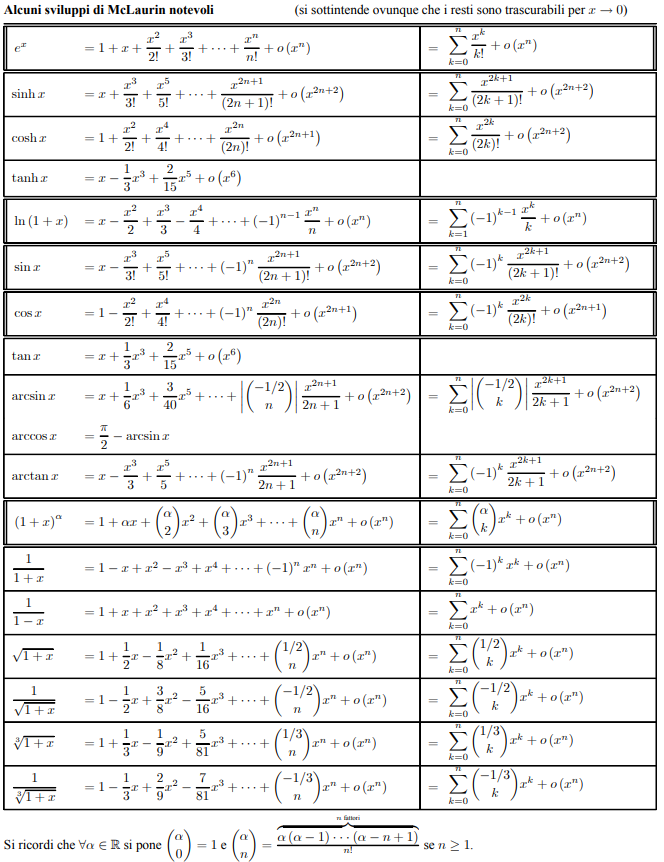
\includegraphics[width=\linewidth]{../0-ripasso/mclaurin.PNG}
\end{figure}